\documentclass[10pt,a4paper]{article}
\usepackage[utf8]{inputenc}
\usepackage{amsmath}
\usepackage{amsfonts}
\usepackage{amssymb}
\usepackage{url}
\usepackage{graphicx}
\graphicspath{ {img/} }

\begin{document}

\title{%
  Bee Tracking \\
  \large Computer Vision Systems Programming \\
    Vienna University of Technology}
%\subtitle{asdf}
\author{Dominik Schörkhuber\\dominik@schoerkhuber.net}
\maketitle

\begin{abstract}
Varroa Destructor is a parasite harming bee colonies. As the worldwide bee population is at danger, beekeepers as well as researchers are looking for methods to monitor the health of bee hives. In this work we first analyze given data from a long term video observation [Section~\ref{sec:data}]. In [Section~\ref{sec:method}] we construct an algorithm to identify and track bees. Finally the acquired data material is used to create a new dataset of bee patches which a SVM was trained on [Section~\ref{sec:newdataset}].
\end{abstract}

\section{Introduction}
Since the year 2006 beekeepers have noticed their honeybee populations to decrease at alarming  and increasing rates. The main reason for these mass dyings is the Varroa Destructor mite. This mite is found to attach to the bees and their brood. Most species of honeybees do have no measures to defend themselves against the infestation. The mites can multiply unimpeded and  cripples the newly hatched brood \cite{hagopian}\cite{epstein}.

\begin{figure}
\centering
\includegraphics[width=0.5\textwidth]{crippled}
\caption{Bee with crippled wings, caused by Varroa infection}
\end{figure}

Since the honeybees are not able to fend of the mites, they are dependent on the beekeeper to keep track of infestations. Beekeepers regulary check the hives for mites, and use formic acids (among others) to stem an infestation. However, the mites quickly build up resistances against different used chemicals and the bees are negatively affected to a certain degree too \cite{chiron2013detecting}.

For these reasons it is important to identify infestations early on by constantly monitoring the health of the bee hives. The most simple solution to analyse the health of a colony is to count entering and exiting bees from the hive, this already lets biologists and beekeepers infer information on the healthiness. In this work however we are focussed on the identification and tracking of individual bees, which might for one be used to again count bees, but may also be used for behavioural analysis. Finally we use the created detection and tracking algorithm to propose a new dataset containing beepatches for further machine learning methods.

\section{Related Work}

Chiron et al. state the need for observation of bees to monitor abnormal behaviour, which can be used to diagnose the health state of a hive. In particular they are interested in the number of bees and trajectories. To capture video footage Chiron et al. use a stereo camera system. The available depth information makes it much easier for them to accurately detect the bees. For tracking a Global Nearest Neighbours approach with a Kalman Filter is used \cite{chiron2013detecting}.

Beesbook is a project series by FU Berlin \cite{beesbook}. The beebook observes all bees of a hive in a spatial, temporal and social context. Main goal here is to analyse and understand bee dances. To analyse the dances also an accurate tracking is needed. Wario et al. solve this problem with a marker based tracking \cite{wario2015automatic}. 

Finally the company Keltronixinc is marketing bee monitoring as a service \cite{keltronixinc}. The system consists of a camera and computer which is setup at the bee hive. The camera is looking at the beehive and monitors the bee activity with a tracking algorithm. Keltronixinc claims that they can distinguish between healthy and not healthy hives by analysing activity patterns.

\section{Data Material}
\label{sec:data}

Long-time outdoor video observation in an uncontrolled environment is a very difficult task. For one the bees are very small targets and environmental influences, mainly weather and lighting conditions, make long term observations complex and costly. The data used in this work has therefore been acquired in a more constrained environment (Missing reference).

\begin{figure}
\label{fig:beeentrance}
\centering
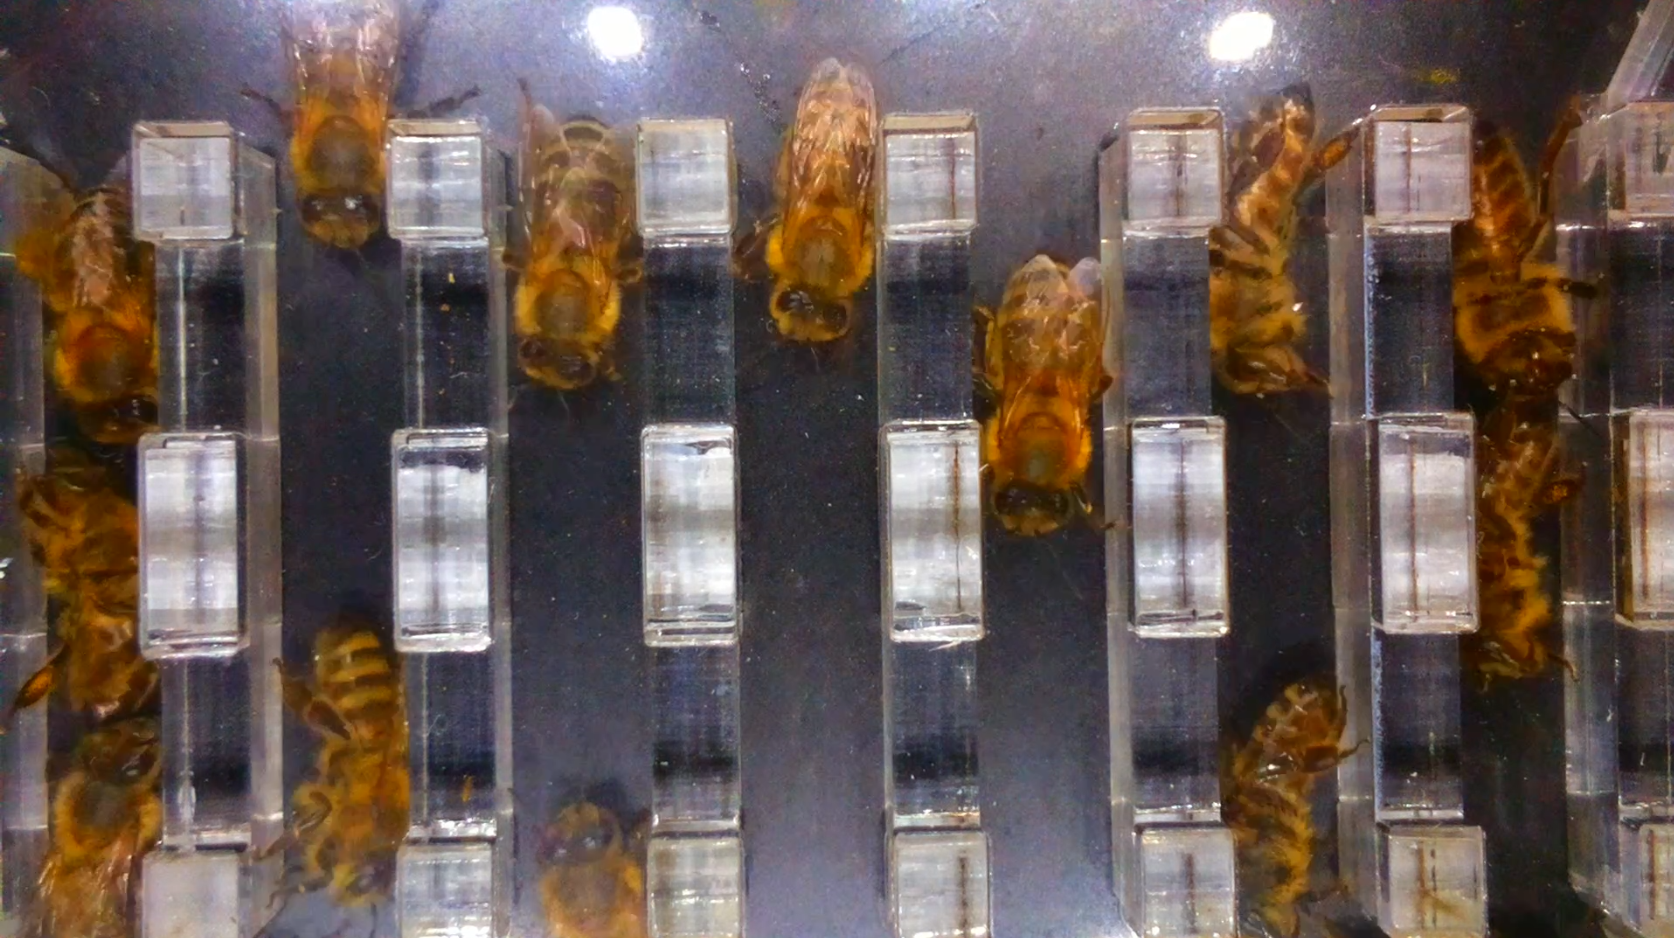
\includegraphics[width=0.5\textwidth]{datasample}
\caption{Example snapshot from the video footage. Shown is a seven lane plexiglass entry for the bees. The entrance is lit by several LED lights to ensure constant lighting conditions}
\end{figure}

At the entrance of the hive a gateway is placed which the bees have to pass while exiting or entering the hive. This narrowing constrains the space to observe and also gives better control over lighting conditions. Figure~\ref{fig:beeentrance} shows the surveilled entrance.  

Across all video material we received, the camera is very stable. This means it is much easier to build effective background models. Another very positive property across all images is the color saturation which nicely separates the bees from the background.

While detection and tracking are a way more well posed problem than in any related work before we had found, it still poses some challenges to the applied video processing algorithms.

\paragraph{Observed Problems} 
At first glance the lighting looks very consistent in the provided videos. However, that is not really the case, neither temporally nor spatially. First to observe are the LED lights illuminating the scene. Depending on the exact positioning of the camera each light can produce a bright highlight disturbing video processing algorithms. The highlights could probably moved out of the cameras field of view, or the LEDs themselves might be positioned further from the ground.

Secondly the lights are also changing with approximately $0.5Hz$ from red to blue. That could be an artefact from pulse width modulating the lights. 

Furthermore the plexiglass walls are problematic. Especially the vertical walls are reflecting a lot of color from the bees, that makes it difficult to categorize pixels into foreground and background just based on their colors. This problem is of course in conjunction with the cameras perspective, as the center lane does not suffer from this. Here the vertical walls are barely visible, the further we move to the left or right, the more reflections on the walls are visible. 

Especially the right most lane was a problematic in many videos because of its much darker lighting, and big angle.

\section{Bee Tracking Algorithm}
\label{sec:method}

In this section we are going to present our new detection and tracking algorithm. On a higher level the algorithm tries to detect bees in each frame. When a suitable detection has been observed the algorithm may start a new tracker on that position. Several rules ensure the tracking stability and control the generation and destruction of trackers. 

\subsection{Detection}
The input data has a fairly high resolution of 1920x1080 pixels. In a first step we arbitrarily chose to reduce the resolution to 30\% as the high resolution does not give us any additional information but slows down computation. As mentioned in Section~\ref{sec:data} the image saturation is a fairly distinctive feature to separate the bees from the background. See Figure~\ref{fig:hsvbee} for an example.

\begin{figure}
\label{fig:hsvbee}
\centering
\includegraphics[width=0.5\textwidth]{hsvbee}
\caption{Image of a bee transformed into HSV color space. The false-color image shows the image saturation in the green channel. It seems to be a fairly distinctive feature to separate bees from the background.}
\end{figure}

A threshold is applied to the saturation image to separate foreground and background of the video frames. Morphological closing helps to produce more consistent blobs. Furthermore we apply a hole closing algorithm to further improve the blob quality. Figure~\ref{fig:preprocessing} shows the resulting image after preprocessing with Closing and Holefilling. 

\begin{figure}
\label{fig:preprocessing}
\center
\includegraphics[width=1.2\textwidth]{preprocessing}
\caption{Top left: Thresholding applied to saturation image. Top right: Image after preprocessing with Morphological Closing and Hole Filling algorithm. Bottom: Final image showing the detections and trackers.}
\end{figure}

The hole filling works as follows. First we start to floodfill the thresholded image visible in \ref{fig:preprocessing} top left. We start the floodfilling from all four image corners, this is not a safe solution, but for the sake of demonstration suitable. Any pixel that is safely classified as background in the image would be suitable to start floodfilling. After flooding the image with white pixels all that remains black are structures enclosed inside white foreground pixels. By inverting the result we get a binary mask where all enclosed pixels, i.e. pixels part of holes, are rendered white. Finally we combine it with the original mask by a bitwise OR operation. The holes are now filled. 

Next we do a connected component analysis on the binary mask. Since bees are very similar in size among each other and the camera distance is constant among all videos, we can safely define the size of a bee in pixels. For each resulting component we take a look at the covered pixel area. If the pixel area is smaller than 800 pixels the blob gets rejected right away. This cleans out most of the noise from reflections on the plexiglass walls. If a blob is bigger than 3500 pixels we assume the detected blob is a fusion of multiple bees. These blobs need to be rejected in a first step too, as we are only interested in single bee detections for the sake of starting a new tracker. If a component meets these conditions the distances to all already established trackers are computed, we then only allow the creation of a new tracker if no other tracker is already within a range of 60 pixels.

\subsection{Tracking}
The tracking of bees happens with a Mean-Shift tracker. Once a tracker is created first a fixed size region of interest is created. We fixed this size to 40x60 pixels as that approximately matches the average bee. Within the tracking window a color histogram is computed which is used in the following video frames by the Mean-Shift tracker to locate the bee. Whenever a bee detection is very close to an established tracker we snap the nearest tracker to that position, as we found the per frame bee detection to be more accurate than the Mean-Shift tracking.

After first tests we noticed two main problems with this kind of tracking. Firstly it is likely to happen that a bee "loses" its tracking window. The window then strands at some static position on the background, and gets picked up by another bee, or resides there forever. Secondly a stranded tracker may be picked up by a bee with a tracker already tracking it. This results in multiple trackers tracking the same bee. A similar problem also appears when two bees get very close. The tracking windows then occasionally tend to jump over to the other bee. That probably happens because the color histograms of two bees are very similar. 

We deal with these cases by validating existing tracking each frame. To prevent tracking windows from loosing their bees we check for foreground pixels within the tracking window area. For perfect detections the amount of foreground pixels within the tracking window should be about 90\% of its size. This can also be seen in \ref{fig:preprocessing} bottom, where the numbers on the bees represent the percentage of foreground pixels. If a tracking window contains less than 25\% foreground pixels we simply destroy the assigned tracker. This also poses as a rather simple solution to destroy trackers that move out of the image area.

Furthermore the distance between each two trackers is validated. For that we store the last time a tracker was snapped to a successful bee detection. This gives us a measure on which of two trackers might be more valid to keep. At a collision of two trackers, the one being more out of date is destroyed.

\subsection{Evaluation}
Evaluation of the tracking algorithm is a difficult task for multiple reasons. The purpose of the algorithm is undefined so we do not know when a correct tracking is crucial. This insecurity already starts with the bee moving through the image border to the inside of the frame. The question arises when an actual tracking needs to start for a bee to be defined as correctly detected. 

For the following evaluation the goal was defined such that a bee must be detect once it fully moved inside one of the seven lanes. We did a manual counting on how many bees had been detected correctly (i.e. tracking window is in the correct position) each frame (TP), how many detections happened without a bee present (FP) and how many bees were not detected (FN) on a per frame basis. 

For the evaluation one video was randomly selected and manually counted by the above defined measures. Results are TP: 1409, FP: 35, FN: 21, F1: 0.98

At this point it needs to be again emphasized that these numbers need to be put into perspective with the application such a tracker would be used in.

\section{Dataset for Machine Learning}
\label{sec:newdataset}
The algorithm designed in previous sections is a very specialised one to the given environment. With the change of lighting conditions, camera distance or other variables this algorithm may not be robust enough to provide consistent tracking. It would be therefore desirable to create more flexible algorithms based on machine learning. 

In this section we present an approach to first extract data from the new detection and tracking algorithm. Finally we experiment with a Support Vector Machine to detect bees. The following approach was published by Dalal et al. \cite{dalal2005histograms}, and is based on first extracting numerous image patches of training data. Histogram of Gradients features are extracted from the patches. Then a Support Vector Machine is trained on those features. To finally detect subjects in an image, the image is processed with a sliding window approach. Each position of the sliding window is classified by the Support Vector Machine. See \ref{fig:svmresult} for the achieved output of our classifier. 

\begin{figure}
\label{fig:preprocessing}
\center
\includegraphics[width=1.0\textwidth]{svmresult}
\caption{Image after sliding window classification of the trained support vector machine.}
\end{figure}

\subsection{Creating a Dataset}
With having the per frame detections of the tracking algorithm we are able to locate the bees and extract them into image patches. For our purposes we chose a fixed patch size of 64x128 pixels, which will be later on beneficial for the used Histogram of Gradients descriptor. The tracker positions are further validated before extracting the patch positions. Tracker positions are only accepted for extraction if they contain more than 90\% foreground pixels, further restrictions may be specified at this point e.g. putting restrictions on the distances between tracking windows may be beneficial too.

Similarly negative examples have been extracted. First we compute an average image over a whole input video. This results in a pretty clear background image already, but on very crowded videos smears are visible. Because of that we additionally mask out pixels by thresholding the saturation image, and then do a weighted averaging. From this background image negative samples are extracted with a sliding window.

\begin{figure}
\label{fig:datasetsample}
\center
\includegraphics[width=1.0\textwidth]{datasetsample}
\caption{Extracted image patches for positive and negative examples.}
\end{figure}

\subsection{Training and Classification} 
To feed the extracted image patches into a Support Vector Machine we are first computing a feature representation of each patch. This is done by a Histogram of Gradient algorithm which splits each 64x128 patch into 8x8 pixel cells. A block is defined as 16x16 pixels big, for each block a histogram of gradient directions with 16 bins is computed. That means each patch contains 7x15 blocks, each containing 4 histograms with 16 values. Combined this results in a descriptor with 6720 values. 

For classification a sliding windows approach is used, where each position of the sliding window is classfied on its own. Figure~\ref{fig:svmresult} shows the resulting detections in red. Since the image was cluttered with too many detections we additionally used a simple non-maxima suppression which reduces the number of detections considerably, shown in green.

Apparently the SVM has learned to detect bees to some degree, whereas the result is way less accurate than the original algorithm. 

\section{Conclusion}
In this work we have created a detection and tracking algorithm for a specialised bee observation setup. Furthermore we used the algorithm to generate a new patch-based bee dataset, for applications of machine learning, and trained a simple model on the dataset to detect bees in the originally provided video footage.

We hope that the generated data will be of use for future detection and tracking algorithms, and lets future researchers create more robust tracking algorithms with it.

\bibliography{finalreport}
\bibliographystyle{alpha}
\end{document}